\documentclass{article}\usepackage[]{graphicx}\usepackage[]{color}
%% maxwidth is the original width if it is less than linewidth
%% otherwise use linewidth (to make sure the graphics do not exceed the margin)
\makeatletter
\def\maxwidth{ %
  \ifdim\Gin@nat@width>\linewidth
    \linewidth
  \else
    \Gin@nat@width
  \fi
}
\makeatother

\definecolor{fgcolor}{rgb}{0.345, 0.345, 0.345}
\newcommand{\hlnum}[1]{\textcolor[rgb]{0.686,0.059,0.569}{#1}}%
\newcommand{\hlstr}[1]{\textcolor[rgb]{0.192,0.494,0.8}{#1}}%
\newcommand{\hlcom}[1]{\textcolor[rgb]{0.678,0.584,0.686}{\textit{#1}}}%
\newcommand{\hlopt}[1]{\textcolor[rgb]{0,0,0}{#1}}%
\newcommand{\hlstd}[1]{\textcolor[rgb]{0.345,0.345,0.345}{#1}}%
\newcommand{\hlkwa}[1]{\textcolor[rgb]{0.161,0.373,0.58}{\textbf{#1}}}%
\newcommand{\hlkwb}[1]{\textcolor[rgb]{0.69,0.353,0.396}{#1}}%
\newcommand{\hlkwc}[1]{\textcolor[rgb]{0.333,0.667,0.333}{#1}}%
\newcommand{\hlkwd}[1]{\textcolor[rgb]{0.737,0.353,0.396}{\textbf{#1}}}%
\let\hlipl\hlkwb

\usepackage{framed}
\makeatletter
\newenvironment{kframe}{%
 \def\at@end@of@kframe{}%
 \ifinner\ifhmode%
  \def\at@end@of@kframe{\end{minipage}}%
  \begin{minipage}{\columnwidth}%
 \fi\fi%
 \def\FrameCommand##1{\hskip\@totalleftmargin \hskip-\fboxsep
 \colorbox{shadecolor}{##1}\hskip-\fboxsep
     % There is no \\@totalrightmargin, so:
     \hskip-\linewidth \hskip-\@totalleftmargin \hskip\columnwidth}%
 \MakeFramed {\advance\hsize-\width
   \@totalleftmargin\z@ \linewidth\hsize
   \@setminipage}}%
 {\par\unskip\endMakeFramed%
 \at@end@of@kframe}
\makeatother

\definecolor{shadecolor}{rgb}{.97, .97, .97}
\definecolor{messagecolor}{rgb}{0, 0, 0}
\definecolor{warningcolor}{rgb}{1, 0, 1}
\definecolor{errorcolor}{rgb}{1, 0, 0}
\newenvironment{knitrout}{}{} % an empty environment to be redefined in TeX

\usepackage{alltt}
\usepackage{amscd, amssymb, amsmath, verbatim, setspace}
\usepackage[left=1.0in, right=1.0in, top=1.0in, bottom=1.0in]{geometry}
\usepackage{mathrsfs}
\usepackage{listings}


\IfFileExists{upquote.sty}{\usepackage{upquote}}{}
\begin{document}
\begin{flushright}
Arif Ali\\
Math 611 Stochastic Simulation\\
Nov 10, 2016\\
\end{flushright}

\begin{center}
\LARGE\textbf{Homework 9}
  \end{center}
\section*{Exercise 1}
\begin{equation}
P(N(s)=m|N(t)=n)=\left(\begin{array}{c}
n\\
m
\end{array}\right)\left(\frac{s}{t}\right)^{m}\left(1-\frac{s}{t}\right)^{n-m}
\end{equation}
\section*{Exercise 2}
\begin{equation}
P(T>t)=P(Bus_{A}>t)P(Bus_{B}>t)=e^{-2t}*e^{-t}=e^{-3t}
\end{equation}
\section*{Exercise 3}
\begin{knitrout}
\definecolor{shadecolor}{rgb}{0.969, 0.969, 0.969}\color{fgcolor}\begin{kframe}
\begin{alltt}
\hlstd{log_f} \hlkwb{=} \hlkwa{function}\hlstd{(}\hlkwc{y}\hlstd{,}\hlkwc{n}\hlstd{=}\hlnum{101}\hlstd{)\{}
  \hlopt{-}\hlstd{y}\hlopt{+}\hlstd{(n}\hlopt{-}\hlnum{1}\hlstd{)}\hlopt{/}\hlnum{2}\hlopt{*}\hlkwd{log}\hlstd{(}\hlnum{1}\hlopt{-}\hlkwd{exp}\hlstd{(}\hlopt{-}\hlstd{y))}\hlopt{+}\hlstd{(}\hlopt{-}\hlstd{y}\hlopt{*}\hlstd{(n}\hlopt{-}\hlnum{1}\hlstd{)}\hlopt{/}\hlnum{2}\hlstd{)}
\hlstd{\}}

\hlstd{RWMH} \hlkwb{=} \hlkwa{function}\hlstd{(}\hlkwc{S}\hlstd{,} \hlkwc{x0}\hlstd{=}\hlnum{1}\hlstd{,} \hlkwc{N} \hlstd{=} \hlnum{1e4}\hlstd{)\{}
  \hlstd{x} \hlkwb{=} \hlstd{x0}
  \hlstd{accept} \hlkwb{=} \hlnum{0}
  \hlstd{means} \hlkwb{=} \hlstd{x0}
  \hlkwa{for}\hlstd{(t} \hlkwa{in} \hlnum{2}\hlopt{:}\hlstd{N)\{}
    \hlstd{y} \hlkwb{=} \hlkwd{rnorm}\hlstd{(}\hlnum{1}\hlstd{, x[t}\hlopt{-}\hlnum{1}\hlstd{], S)}
    \hlstd{accept[t]} \hlkwb{=} \hlnum{0}
    \hlstd{x[t]} \hlkwb{=}\hlstd{x[t}\hlopt{-}\hlnum{1}\hlstd{]}
    \hlstd{rho} \hlkwb{=} \hlkwd{exp}\hlstd{(}\hlkwd{log_f}\hlstd{(y))}\hlopt{/}\hlkwd{exp}\hlstd{(}\hlkwd{log_f}\hlstd{(x[t}\hlopt{-}\hlnum{1}\hlstd{]))}
    \hlstd{u} \hlkwb{=} \hlkwd{runif}\hlstd{(}\hlnum{1}\hlstd{)}
      \hlkwa{if}\hlstd{(}\hlopt{!}\hlkwd{is.na}\hlstd{(rho))\{}
        \hlkwa{if}\hlstd{(u}\hlopt{<}\hlstd{rho)\{}
          \hlstd{x[t]} \hlkwb{=} \hlstd{y}
          \hlstd{accept[t]} \hlkwb{=} \hlnum{1}

          \hlstd{\}}
      \hlstd{\}}
    \hlstd{means[t]} \hlkwb{=} \hlkwd{mean}\hlstd{(x)}
  \hlstd{\}}
  \hlkwd{return}\hlstd{(}\hlkwd{data.frame}\hlstd{(x, accept, means))}
  \hlstd{\}}
\end{alltt}
\end{kframe}
\end{knitrout}
\section*{Exercise 4}
\begin{knitrout}
\definecolor{shadecolor}{rgb}{0.969, 0.969, 0.969}\color{fgcolor}\begin{kframe}
\begin{alltt}
\hlstd{S_1} \hlkwb{=} \hlkwd{RWMH}\hlstd{(}\hlnum{1}\hlstd{)}
\hlkwd{mean}\hlstd{(S_1}\hlopt{$}\hlstd{accept)}
\end{alltt}
\begin{verbatim}
## [1] 0.131
\end{verbatim}
\begin{alltt}
\hlkwd{plot}\hlstd{(S_1}\hlopt{$}\hlstd{x,} \hlkwc{type}\hlstd{=}\hlstr{"l"}\hlstd{,}
       \hlkwc{ylab}\hlstd{=}\hlstr{"X"}\hlstd{,} \hlkwc{ylim}\hlstd{=}\hlkwd{range}\hlstd{(S_1}\hlopt{$}\hlstd{x),} \hlkwc{main} \hlstd{=} \hlstr{"Sampled Values"}\hlstd{)}
\end{alltt}
\end{kframe}
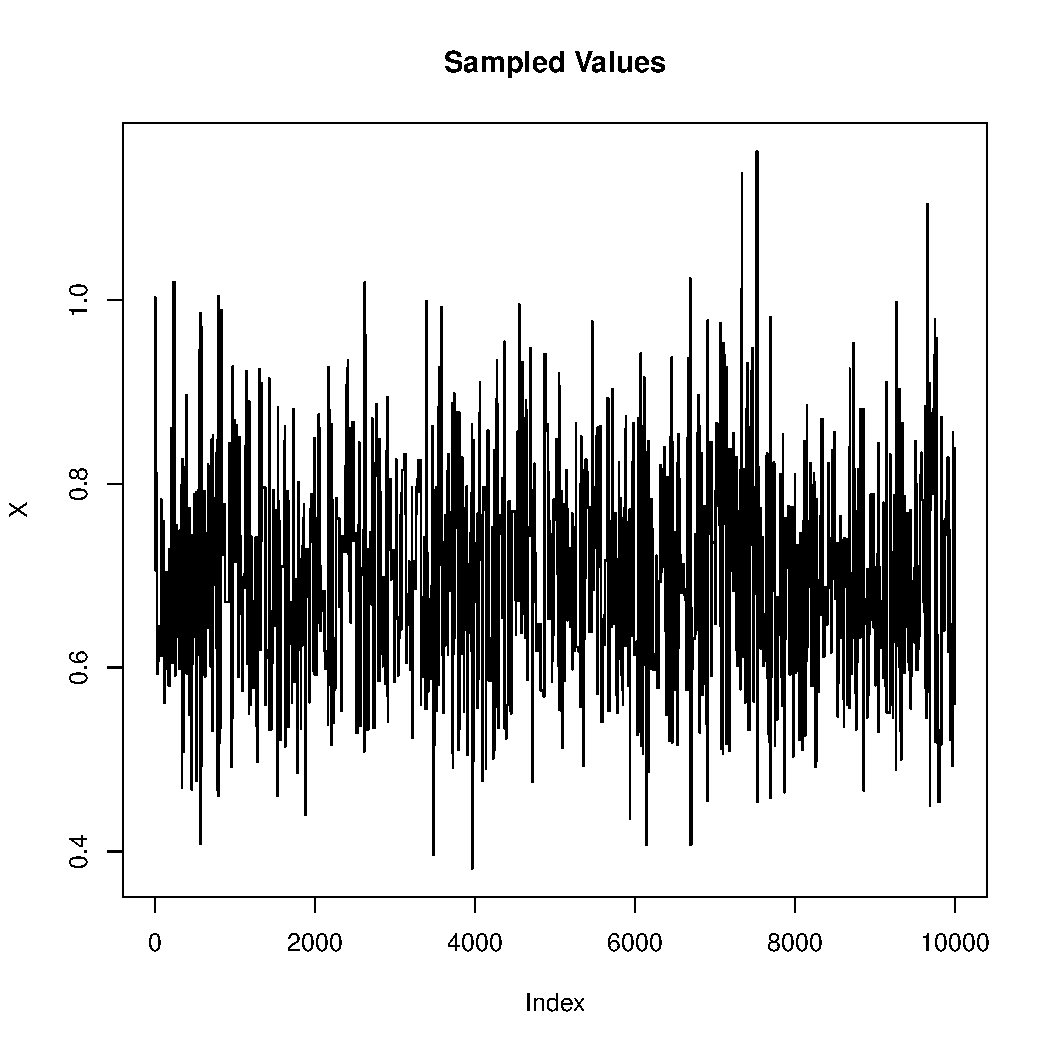
\includegraphics[width=0.60\linewidth]{figure/unnamed-chunk-3-1} 
\begin{kframe}\begin{alltt}
\hlkwd{plot}\hlstd{(S_1}\hlopt{$}\hlstd{means,} \hlkwc{type}\hlstd{=}\hlstr{"l"}\hlstd{,}
       \hlkwc{ylab}\hlstd{=}\hlstr{"X"}\hlstd{,} \hlkwc{ylim}\hlstd{=}\hlkwd{range}\hlstd{(S_1}\hlopt{$}\hlstd{means),} \hlkwc{main} \hlstd{=} \hlstr{"Sampled Means"}\hlstd{)}
\end{alltt}
\end{kframe}
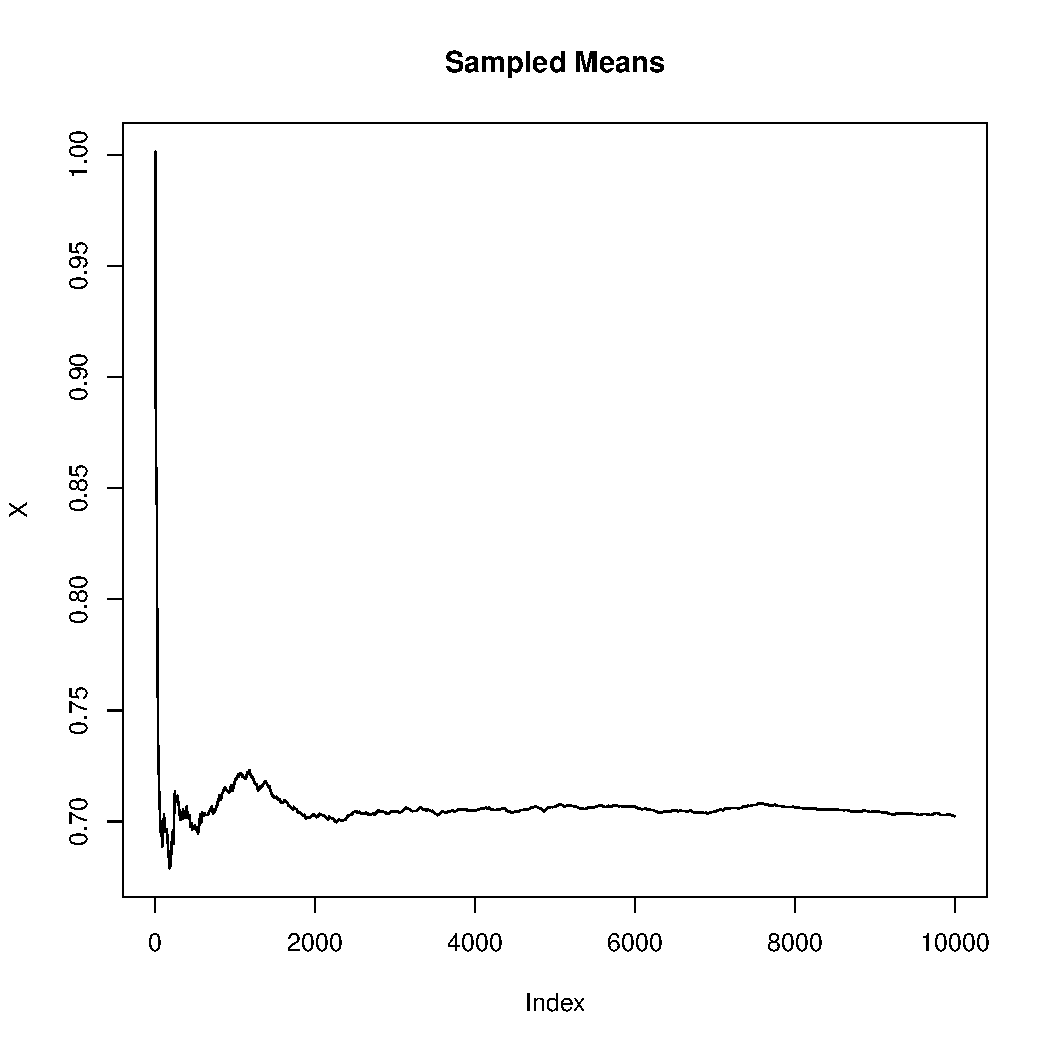
\includegraphics[width=0.60\linewidth]{figure/unnamed-chunk-3-2} 

\end{knitrout}
With $\sigma = 1$, the acceptance rate is very low. This is due most likely because of candidate values that are less than zero. If these values are less than zero, there is no way for them to be within the proposal distribution, thus causing the rejection to occur. The Sampled value graphs seem to indicate that there is a pattern, which means there is some form of convengence. The sample mean seems to hold at approximately the same value after RWHM a run for less than 1000 iterations.  
\begin{knitrout}
\definecolor{shadecolor}{rgb}{0.969, 0.969, 0.969}\color{fgcolor}\begin{kframe}
\begin{alltt}
\hlstd{S_0.1} \hlkwb{=} \hlkwd{RWMH}\hlstd{(}\hlnum{0.1}\hlstd{)}
\hlkwd{mean}\hlstd{(S_0.1}\hlopt{$}\hlstd{accept)}
\end{alltt}
\begin{verbatim}
## [1] 0.698
\end{verbatim}
\begin{alltt}
\hlkwd{plot}\hlstd{(S_0.1}\hlopt{$}\hlstd{x,} \hlkwc{type}\hlstd{=}\hlstr{"l"}\hlstd{,}
       \hlkwc{ylab}\hlstd{=}\hlstr{"X"}\hlstd{,} \hlkwc{ylim}\hlstd{=}\hlkwd{range}\hlstd{(S_0.1}\hlopt{$}\hlstd{x))}
\end{alltt}
\end{kframe}
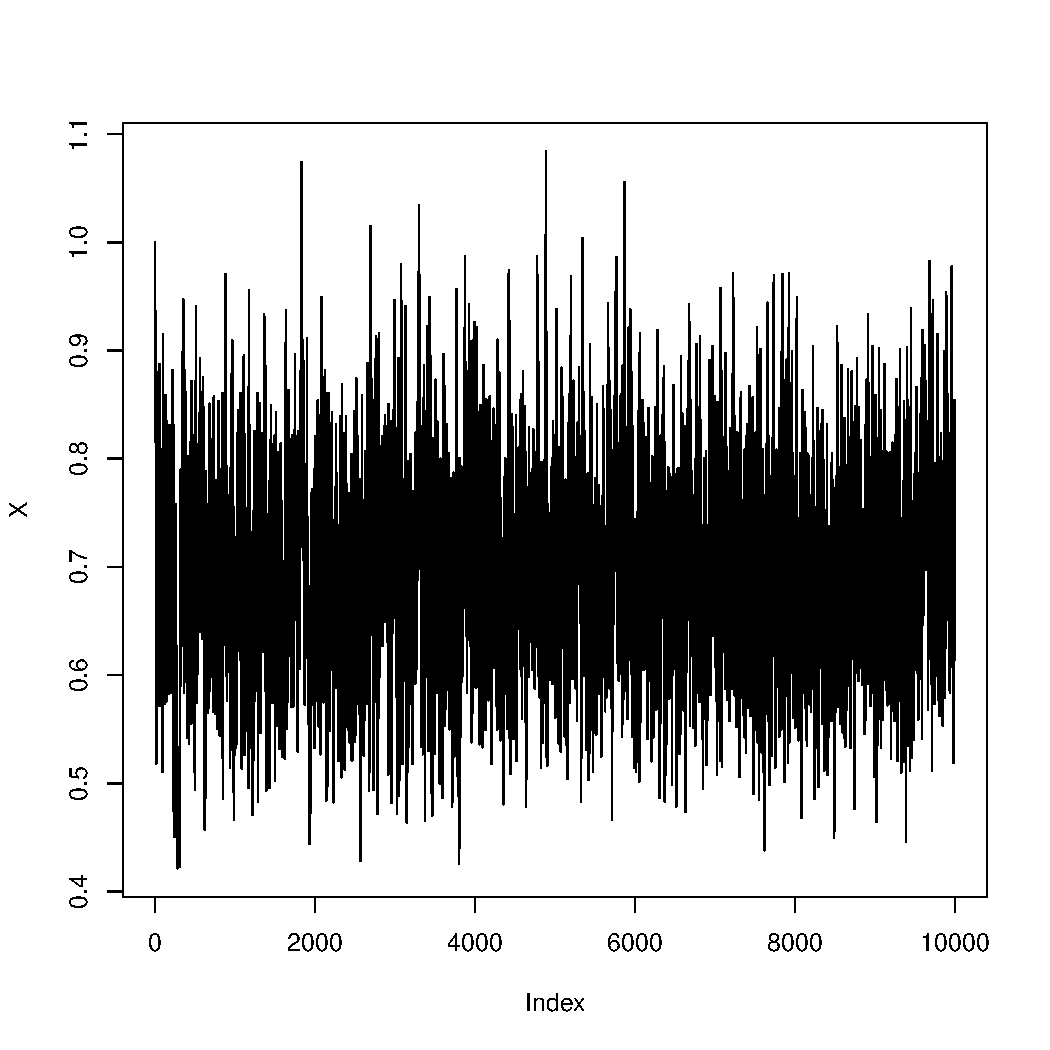
\includegraphics[width=0.60\linewidth]{figure/unnamed-chunk-4-1} 
\begin{kframe}\begin{alltt}
\hlkwd{plot}\hlstd{(S_0.1}\hlopt{$}\hlstd{means,} \hlkwc{type}\hlstd{=}\hlstr{"l"}\hlstd{,}
       \hlkwc{ylab}\hlstd{=}\hlstr{"X"}\hlstd{,} \hlkwc{ylim}\hlstd{=}\hlkwd{range}\hlstd{(S_0.1}\hlopt{$}\hlstd{means),} \hlkwc{main} \hlstd{=} \hlstr{"Sampled Means"}\hlstd{)}
\end{alltt}
\end{kframe}
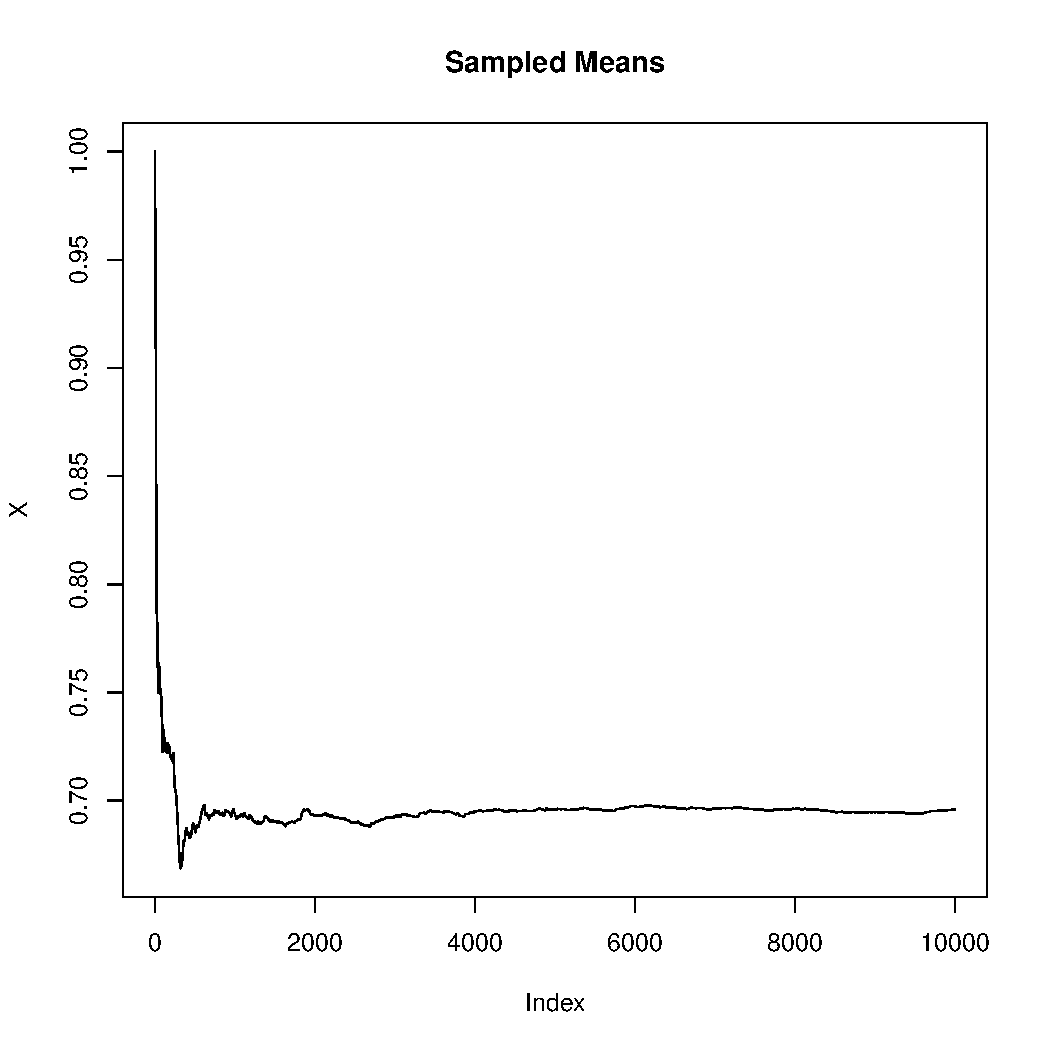
\includegraphics[width=0.60\linewidth]{figure/unnamed-chunk-4-2} 

\end{knitrout}
With $\sigma = 0.1$, the acceptance rate is signicantly greater than the rate when $\sigma = 1$. The patterns indicate convergence, but based on the graph of the Sampled Means, the means seem to hold after less iterations compared to $\sigma = 1$.

\section*{Exercise 5}

\subsection*{uniform}
\begin{knitrout}
\definecolor{shadecolor}{rgb}{0.969, 0.969, 0.969}\color{fgcolor}\begin{kframe}
\begin{alltt}
\hlstd{RWMH} \hlkwb{=} \hlkwa{function}\hlstd{(}\hlkwc{f}\hlstd{)\{}
  \hlstd{N} \hlkwb{=} \hlnum{1e4}
\hlstd{x} \hlkwb{=} \hlnum{1}
\hlstd{accept} \hlkwb{=} \hlnum{0}
\hlstd{means} \hlkwb{=} \hlnum{1}
\hlkwa{for}\hlstd{(t} \hlkwa{in} \hlnum{2}\hlopt{:}\hlstd{N)\{}
  \hlstd{y} \hlkwb{=} \hlkwd{f}\hlstd{(x[t}\hlopt{-}\hlnum{1}\hlstd{])}
  \hlstd{accept[t]} \hlkwb{=} \hlnum{0}
  \hlstd{x[t]} \hlkwb{=}\hlstd{x[t}\hlopt{-}\hlnum{1}\hlstd{]}
  \hlstd{rho} \hlkwb{=} \hlkwd{dnorm}\hlstd{(y,}\hlnum{0}\hlstd{,}\hlnum{1}\hlstd{)}\hlopt{/}\hlkwd{dnorm}\hlstd{(x[t}\hlopt{-}\hlnum{1}\hlstd{],}\hlnum{0}\hlstd{,}\hlnum{1}\hlstd{)}
  \hlstd{u} \hlkwb{=} \hlkwd{runif}\hlstd{(}\hlnum{1}\hlstd{)}
      \hlkwa{if}\hlstd{(u}\hlopt{<}\hlstd{rho)\{}
        \hlstd{x[t]} \hlkwb{=} \hlstd{y}
        \hlstd{accept[t]} \hlkwb{=} \hlnum{1}

        \hlstd{\}}
  \hlstd{means[t]} \hlkwb{=} \hlkwd{mean}\hlstd{(x)}
\hlstd{\}}
  \hlkwd{return}\hlstd{(}\hlkwd{data.frame}\hlstd{(x, accept, means))}
\hlstd{\}}

\hlstd{unif_RWMH} \hlkwb{=} \hlkwd{RWMH}\hlstd{(}\hlkwa{function}\hlstd{(}\hlkwc{x}\hlstd{)} \hlkwd{runif}\hlstd{(}\hlnum{1}\hlstd{, x}\hlopt{-}\hlnum{1}\hlstd{, x}\hlopt{+}\hlnum{1}\hlstd{))}
\end{alltt}
\end{kframe}
\end{knitrout}
The acceptance rate for the uniform distribution 80.03\%.
\subsection*{cauchy}
\begin{knitrout}
\definecolor{shadecolor}{rgb}{0.969, 0.969, 0.969}\color{fgcolor}\begin{kframe}
\begin{alltt}
\hlstd{RWMH_cauchy} \hlkwb{=} \hlkwd{RWMH}\hlstd{(}\hlkwa{function}\hlstd{(}\hlkwc{x}\hlstd{)} \hlkwd{rcauchy}\hlstd{(}\hlnum{1}\hlstd{,} \hlkwc{location} \hlstd{= x))}
\hlkwd{plot}\hlstd{(}\hlkwd{density}\hlstd{(RWMH_cauchy}\hlopt{$}\hlstd{x),} \hlkwc{main} \hlstd{=} \hlstr{"Cauchy"}\hlstd{)}
\hlkwd{lines}\hlstd{(}\hlkwd{density}\hlstd{(unif_RWMH}\hlopt{$}\hlstd{x),} \hlkwc{col} \hlstd{=} \hlstr{"red"}\hlstd{)}
\hlkwd{legend}\hlstd{(}\hlstr{"topright"}\hlstd{,} \hlkwc{legend} \hlstd{=} \hlkwd{c}\hlstd{(}\hlstr{"Cauchy"}\hlstd{,} \hlstr{"uniform"}\hlstd{),} \hlkwc{fill} \hlstd{=} \hlkwd{c}\hlstd{(}\hlstr{"black"}\hlstd{,} \hlstr{"red"}\hlstd{))}
\end{alltt}
\end{kframe}
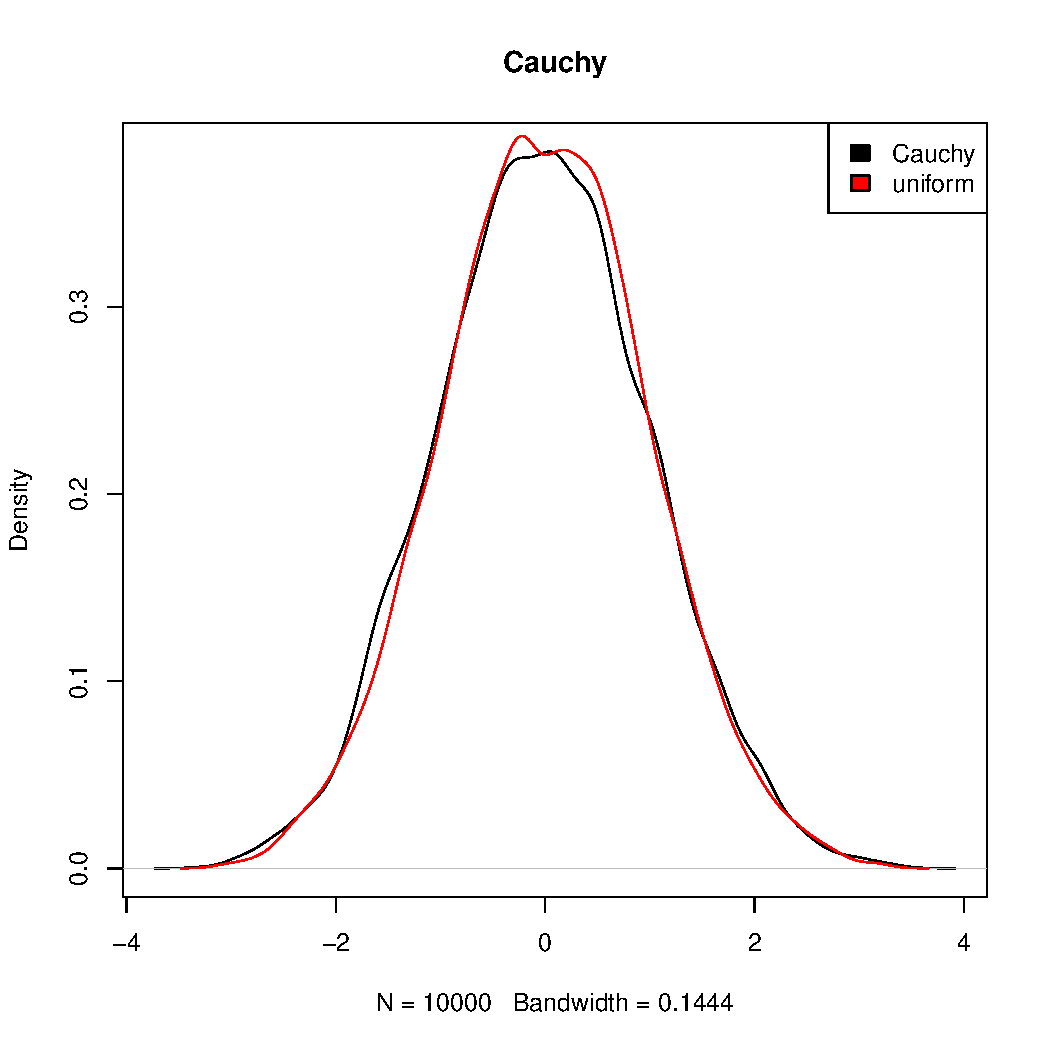
\includegraphics[width=0.60\linewidth]{figure/unnamed-chunk-6-1} 

\end{knitrout}
The acceptance rate for the cauchy distribution 53.86\%. The Cauchy distribution seems  to fit the uniform very closely. This could indicate that the cauchy distribution and uniform distribution are similar candidates for the normal distribution.

\subsection*{laplace}
\begin{knitrout}
\definecolor{shadecolor}{rgb}{0.969, 0.969, 0.969}\color{fgcolor}\begin{kframe}
\begin{alltt}
\hlkwd{library}\hlstd{(smoothmest)}
\end{alltt}


{\ttfamily\noindent\itshape\color{messagecolor}{\#\# Loading required package: MASS}}\begin{alltt}
\hlstd{RWMH_laplace} \hlkwb{=} \hlkwd{RWMH}\hlstd{(}\hlkwa{function}\hlstd{(}\hlkwc{x}\hlstd{)} \hlkwd{rdoublex}\hlstd{(}\hlnum{1}\hlstd{,x))}
\hlkwd{plot}\hlstd{(}\hlkwd{density}\hlstd{(RWMH_laplace}\hlopt{$}\hlstd{x),} \hlkwc{main} \hlstd{=} \hlstr{"Laplace"}\hlstd{)}
\hlkwd{lines}\hlstd{(}\hlkwd{density}\hlstd{(unif_RWMH}\hlopt{$}\hlstd{x),} \hlkwc{col} \hlstd{=} \hlstr{"red"}\hlstd{)}
\hlkwd{legend}\hlstd{(}\hlstr{"topright"}\hlstd{,} \hlkwc{legend} \hlstd{=} \hlkwd{c}\hlstd{(}\hlstr{"laplace"}\hlstd{,} \hlstr{"uniform"}\hlstd{),} \hlkwc{fill} \hlstd{=} \hlkwd{c}\hlstd{(}\hlstr{"black"}\hlstd{,} \hlstr{"red"}\hlstd{))}
\end{alltt}
\end{kframe}
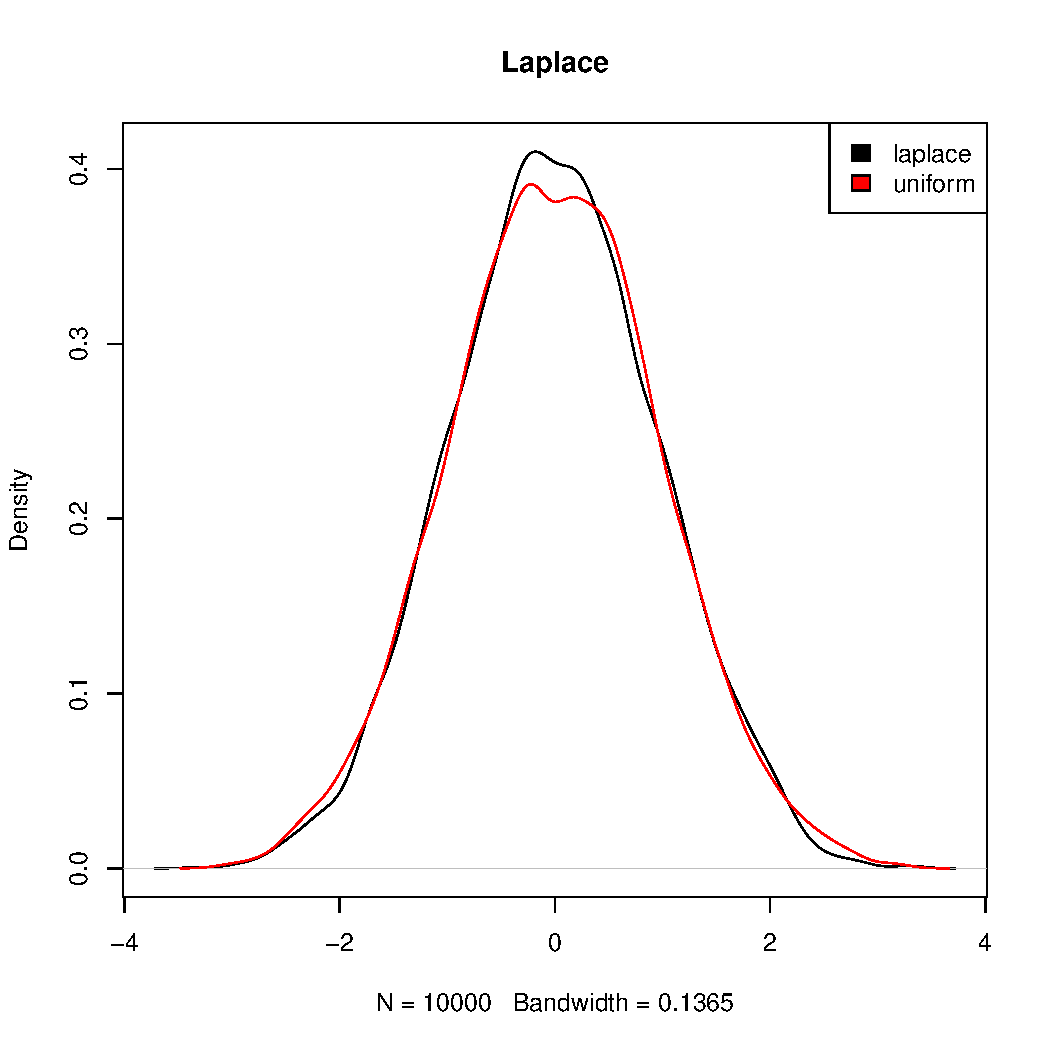
\includegraphics[width=0.60\linewidth]{figure/unnamed-chunk-8-1} 

\end{knitrout}
The acceptance rate for the laplace distribution 65.94\%. Unlike the Cauchy distribution, there seem to be more noticable differences especially at the peak of the distributions. 
\subsection*{laplace vs cauchy}
\begin{knitrout}
\definecolor{shadecolor}{rgb}{0.969, 0.969, 0.969}\color{fgcolor}\begin{kframe}
\begin{alltt}
\hlkwd{plot}\hlstd{(}\hlkwd{density}\hlstd{(RWMH_cauchy}\hlopt{$}\hlstd{x),} \hlkwc{main} \hlstd{=} \hlstr{"Cauchy vs Laplace"}\hlstd{)}
\hlkwd{lines}\hlstd{(}\hlkwd{density}\hlstd{(RWMH_laplace}\hlopt{$}\hlstd{x),} \hlkwc{col} \hlstd{=} \hlstr{"red"}\hlstd{)}
\hlkwd{legend}\hlstd{(}\hlstr{"topright"}\hlstd{,} \hlkwc{legend} \hlstd{=} \hlkwd{c}\hlstd{(}\hlstr{"cauchy"}\hlstd{,} \hlstr{"laplace"}\hlstd{),} \hlkwc{fill} \hlstd{=} \hlkwd{c}\hlstd{(}\hlstr{"black"}\hlstd{,} \hlstr{"red"}\hlstd{))}
\end{alltt}
\end{kframe}
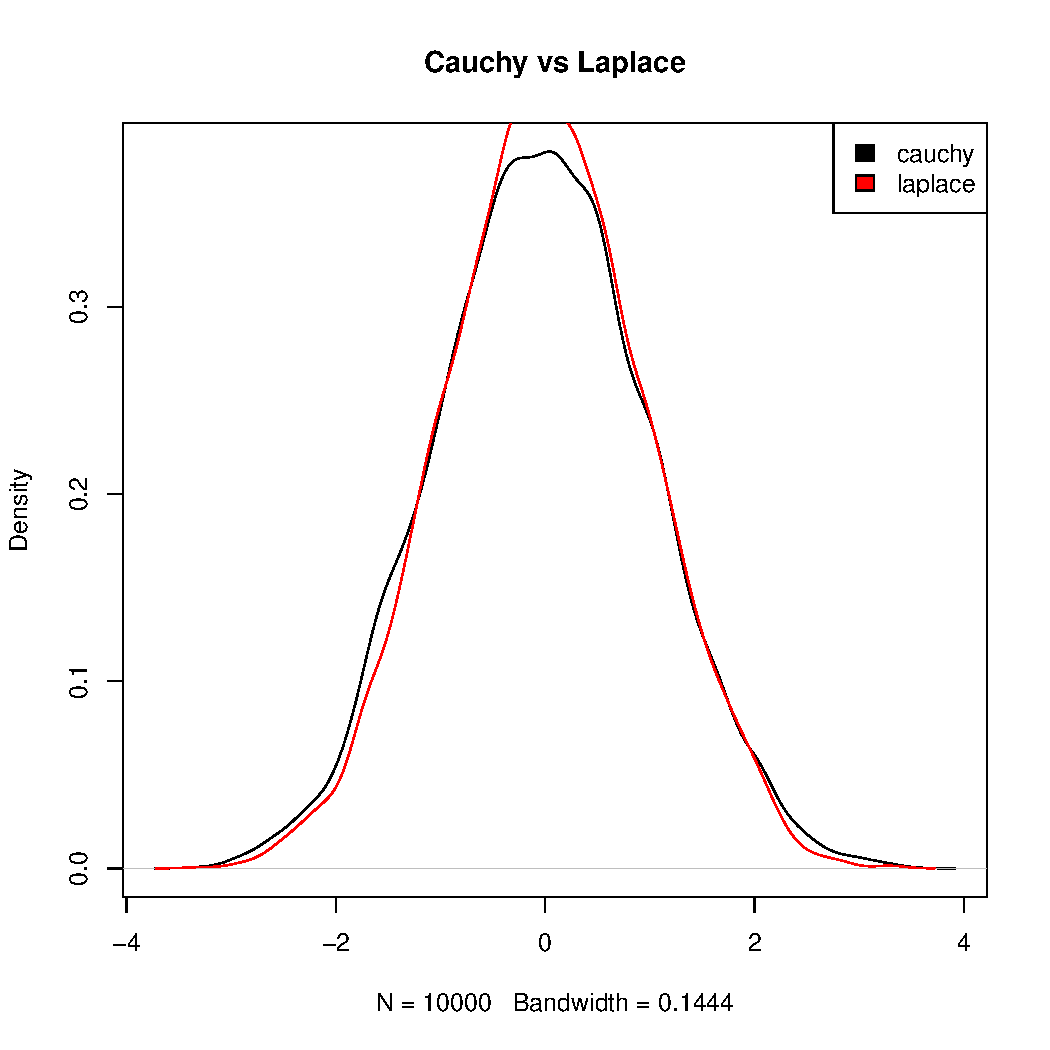
\includegraphics[width=0.60\linewidth]{figure/unnamed-chunk-9-1} 

\end{knitrout}
The results are similiar to the comparisions of the laplace vs uniform distribution.
\begin{knitrout}
\definecolor{shadecolor}{rgb}{0.969, 0.969, 0.969}\color{fgcolor}\begin{kframe}
\begin{alltt}
\hlkwd{plot}\hlstd{(RWMH_cauchy}\hlopt{$}\hlstd{means,} \hlkwc{type} \hlstd{=}\hlstr{"l"}\hlstd{,} \hlkwc{main} \hlstd{=} \hlstr{"Means"}\hlstd{)}
\hlkwd{lines}\hlstd{(RWMH_laplace}\hlopt{$}\hlstd{means,} \hlkwc{col} \hlstd{=} \hlstr{"red"}\hlstd{)}
\hlkwd{legend}\hlstd{(}\hlstr{"topright"}\hlstd{,} \hlkwc{legend} \hlstd{=} \hlkwd{c}\hlstd{(}\hlstr{"cauchy"}\hlstd{,} \hlstr{"laplace"}\hlstd{),} \hlkwc{fill} \hlstd{=} \hlkwd{c}\hlstd{(}\hlstr{"black"}\hlstd{,} \hlstr{"red"}\hlstd{))}
\end{alltt}
\end{kframe}
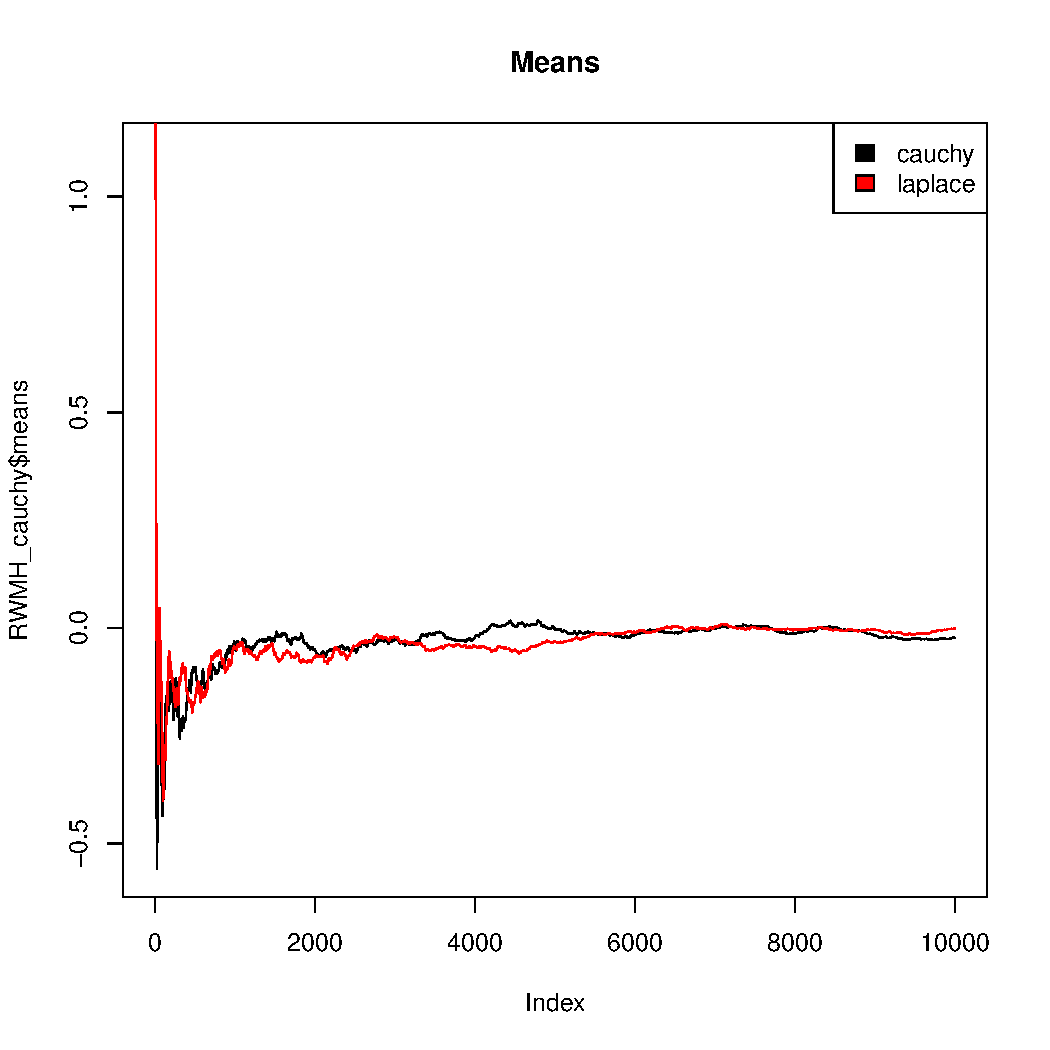
\includegraphics[width=0.60\linewidth]{figure/unnamed-chunk-10-1} 

\end{knitrout}
When comparing the means by iteration of both, it's interesting that it takes the laplace a shorter amount of iterations to reach zero compared to the cauchy distribution. 
\end{document}
